
% Default to the notebook output style

    


% Inherit from the specified cell style.




    
\documentclass[11pt]{article}

    
    
    \usepackage[T1]{fontenc}
    % Nicer default font (+ math font) than Computer Modern for most use cases
    \usepackage{mathpazo}

    % Basic figure setup, for now with no caption control since it's done
    % automatically by Pandoc (which extracts ![](path) syntax from Markdown).
    \usepackage{graphicx}
    % We will generate all images so they have a width \maxwidth. This means
    % that they will get their normal width if they fit onto the page, but
    % are scaled down if they would overflow the margins.
    \makeatletter
    \def\maxwidth{\ifdim\Gin@nat@width>\linewidth\linewidth
    \else\Gin@nat@width\fi}
    \makeatother
    \let\Oldincludegraphics\includegraphics
    % Set max figure width to be 80% of text width, for now hardcoded.
    \renewcommand{\includegraphics}[1]{\Oldincludegraphics[width=.8\maxwidth]{#1}}
    % Ensure that by default, figures have no caption (until we provide a
    % proper Figure object with a Caption API and a way to capture that
    % in the conversion process - todo).
    \usepackage{caption}
    \DeclareCaptionLabelFormat{nolabel}{}
    \captionsetup{labelformat=nolabel}

    \usepackage{adjustbox} % Used to constrain images to a maximum size 
    \usepackage{xcolor} % Allow colors to be defined
    \usepackage{enumerate} % Needed for markdown enumerations to work
    \usepackage{geometry} % Used to adjust the document margins
    \usepackage{amsmath} % Equations
    \usepackage{amssymb} % Equations
    \usepackage{textcomp} % defines textquotesingle
    % Hack from http://tex.stackexchange.com/a/47451/13684:
    \AtBeginDocument{%
        \def\PYZsq{\textquotesingle}% Upright quotes in Pygmentized code
    }
    \usepackage{upquote} % Upright quotes for verbatim code
    \usepackage{eurosym} % defines \euro
    \usepackage[mathletters]{ucs} % Extended unicode (utf-8) support
    \usepackage[utf8x]{inputenc} % Allow utf-8 characters in the tex document
    \usepackage{fancyvrb} % verbatim replacement that allows latex
    \usepackage{grffile} % extends the file name processing of package graphics 
                         % to support a larger range 
    % The hyperref package gives us a pdf with properly built
    % internal navigation ('pdf bookmarks' for the table of contents,
    % internal cross-reference links, web links for URLs, etc.)
    \usepackage{hyperref}
    \usepackage{longtable} % longtable support required by pandoc >1.10
    \usepackage{booktabs}  % table support for pandoc > 1.12.2
    \usepackage[inline]{enumitem} % IRkernel/repr support (it uses the enumerate* environment)
    \usepackage[normalem]{ulem} % ulem is needed to support strikethroughs (\sout)
                                % normalem makes italics be italics, not underlines
    

    
    
    % Colors for the hyperref package
    \definecolor{urlcolor}{rgb}{0,.145,.698}
    \definecolor{linkcolor}{rgb}{.71,0.21,0.01}
    \definecolor{citecolor}{rgb}{.12,.54,.11}

    % ANSI colors
    \definecolor{ansi-black}{HTML}{3E424D}
    \definecolor{ansi-black-intense}{HTML}{282C36}
    \definecolor{ansi-red}{HTML}{E75C58}
    \definecolor{ansi-red-intense}{HTML}{B22B31}
    \definecolor{ansi-green}{HTML}{00A250}
    \definecolor{ansi-green-intense}{HTML}{007427}
    \definecolor{ansi-yellow}{HTML}{DDB62B}
    \definecolor{ansi-yellow-intense}{HTML}{B27D12}
    \definecolor{ansi-blue}{HTML}{208FFB}
    \definecolor{ansi-blue-intense}{HTML}{0065CA}
    \definecolor{ansi-magenta}{HTML}{D160C4}
    \definecolor{ansi-magenta-intense}{HTML}{A03196}
    \definecolor{ansi-cyan}{HTML}{60C6C8}
    \definecolor{ansi-cyan-intense}{HTML}{258F8F}
    \definecolor{ansi-white}{HTML}{C5C1B4}
    \definecolor{ansi-white-intense}{HTML}{A1A6B2}

    % commands and environments needed by pandoc snippets
    % extracted from the output of `pandoc -s`
    \providecommand{\tightlist}{%
      \setlength{\itemsep}{0pt}\setlength{\parskip}{0pt}}
    \DefineVerbatimEnvironment{Highlighting}{Verbatim}{commandchars=\\\{\}}
    % Add ',fontsize=\small' for more characters per line
    \newenvironment{Shaded}{}{}
    \newcommand{\KeywordTok}[1]{\textcolor[rgb]{0.00,0.44,0.13}{\textbf{{#1}}}}
    \newcommand{\DataTypeTok}[1]{\textcolor[rgb]{0.56,0.13,0.00}{{#1}}}
    \newcommand{\DecValTok}[1]{\textcolor[rgb]{0.25,0.63,0.44}{{#1}}}
    \newcommand{\BaseNTok}[1]{\textcolor[rgb]{0.25,0.63,0.44}{{#1}}}
    \newcommand{\FloatTok}[1]{\textcolor[rgb]{0.25,0.63,0.44}{{#1}}}
    \newcommand{\CharTok}[1]{\textcolor[rgb]{0.25,0.44,0.63}{{#1}}}
    \newcommand{\StringTok}[1]{\textcolor[rgb]{0.25,0.44,0.63}{{#1}}}
    \newcommand{\CommentTok}[1]{\textcolor[rgb]{0.38,0.63,0.69}{\textit{{#1}}}}
    \newcommand{\OtherTok}[1]{\textcolor[rgb]{0.00,0.44,0.13}{{#1}}}
    \newcommand{\AlertTok}[1]{\textcolor[rgb]{1.00,0.00,0.00}{\textbf{{#1}}}}
    \newcommand{\FunctionTok}[1]{\textcolor[rgb]{0.02,0.16,0.49}{{#1}}}
    \newcommand{\RegionMarkerTok}[1]{{#1}}
    \newcommand{\ErrorTok}[1]{\textcolor[rgb]{1.00,0.00,0.00}{\textbf{{#1}}}}
    \newcommand{\NormalTok}[1]{{#1}}
    
    % Additional commands for more recent versions of Pandoc
    \newcommand{\ConstantTok}[1]{\textcolor[rgb]{0.53,0.00,0.00}{{#1}}}
    \newcommand{\SpecialCharTok}[1]{\textcolor[rgb]{0.25,0.44,0.63}{{#1}}}
    \newcommand{\VerbatimStringTok}[1]{\textcolor[rgb]{0.25,0.44,0.63}{{#1}}}
    \newcommand{\SpecialStringTok}[1]{\textcolor[rgb]{0.73,0.40,0.53}{{#1}}}
    \newcommand{\ImportTok}[1]{{#1}}
    \newcommand{\DocumentationTok}[1]{\textcolor[rgb]{0.73,0.13,0.13}{\textit{{#1}}}}
    \newcommand{\AnnotationTok}[1]{\textcolor[rgb]{0.38,0.63,0.69}{\textbf{\textit{{#1}}}}}
    \newcommand{\CommentVarTok}[1]{\textcolor[rgb]{0.38,0.63,0.69}{\textbf{\textit{{#1}}}}}
    \newcommand{\VariableTok}[1]{\textcolor[rgb]{0.10,0.09,0.49}{{#1}}}
    \newcommand{\ControlFlowTok}[1]{\textcolor[rgb]{0.00,0.44,0.13}{\textbf{{#1}}}}
    \newcommand{\OperatorTok}[1]{\textcolor[rgb]{0.40,0.40,0.40}{{#1}}}
    \newcommand{\BuiltInTok}[1]{{#1}}
    \newcommand{\ExtensionTok}[1]{{#1}}
    \newcommand{\PreprocessorTok}[1]{\textcolor[rgb]{0.74,0.48,0.00}{{#1}}}
    \newcommand{\AttributeTok}[1]{\textcolor[rgb]{0.49,0.56,0.16}{{#1}}}
    \newcommand{\InformationTok}[1]{\textcolor[rgb]{0.38,0.63,0.69}{\textbf{\textit{{#1}}}}}
    \newcommand{\WarningTok}[1]{\textcolor[rgb]{0.38,0.63,0.69}{\textbf{\textit{{#1}}}}}
    
    
    % Define a nice break command that doesn't care if a line doesn't already
    % exist.
    \def\br{\hspace*{\fill} \\* }
    % Math Jax compatability definitions
    \def\gt{>}
    \def\lt{<}
    % Document parameters
    \title{hw7-soln}
    
    
    

    % Pygments definitions
    
\makeatletter
\def\PY@reset{\let\PY@it=\relax \let\PY@bf=\relax%
    \let\PY@ul=\relax \let\PY@tc=\relax%
    \let\PY@bc=\relax \let\PY@ff=\relax}
\def\PY@tok#1{\csname PY@tok@#1\endcsname}
\def\PY@toks#1+{\ifx\relax#1\empty\else%
    \PY@tok{#1}\expandafter\PY@toks\fi}
\def\PY@do#1{\PY@bc{\PY@tc{\PY@ul{%
    \PY@it{\PY@bf{\PY@ff{#1}}}}}}}
\def\PY#1#2{\PY@reset\PY@toks#1+\relax+\PY@do{#2}}

\expandafter\def\csname PY@tok@w\endcsname{\def\PY@tc##1{\textcolor[rgb]{0.73,0.73,0.73}{##1}}}
\expandafter\def\csname PY@tok@c\endcsname{\let\PY@it=\textit\def\PY@tc##1{\textcolor[rgb]{0.25,0.50,0.50}{##1}}}
\expandafter\def\csname PY@tok@cp\endcsname{\def\PY@tc##1{\textcolor[rgb]{0.74,0.48,0.00}{##1}}}
\expandafter\def\csname PY@tok@k\endcsname{\let\PY@bf=\textbf\def\PY@tc##1{\textcolor[rgb]{0.00,0.50,0.00}{##1}}}
\expandafter\def\csname PY@tok@kp\endcsname{\def\PY@tc##1{\textcolor[rgb]{0.00,0.50,0.00}{##1}}}
\expandafter\def\csname PY@tok@kt\endcsname{\def\PY@tc##1{\textcolor[rgb]{0.69,0.00,0.25}{##1}}}
\expandafter\def\csname PY@tok@o\endcsname{\def\PY@tc##1{\textcolor[rgb]{0.40,0.40,0.40}{##1}}}
\expandafter\def\csname PY@tok@ow\endcsname{\let\PY@bf=\textbf\def\PY@tc##1{\textcolor[rgb]{0.67,0.13,1.00}{##1}}}
\expandafter\def\csname PY@tok@nb\endcsname{\def\PY@tc##1{\textcolor[rgb]{0.00,0.50,0.00}{##1}}}
\expandafter\def\csname PY@tok@nf\endcsname{\def\PY@tc##1{\textcolor[rgb]{0.00,0.00,1.00}{##1}}}
\expandafter\def\csname PY@tok@nc\endcsname{\let\PY@bf=\textbf\def\PY@tc##1{\textcolor[rgb]{0.00,0.00,1.00}{##1}}}
\expandafter\def\csname PY@tok@nn\endcsname{\let\PY@bf=\textbf\def\PY@tc##1{\textcolor[rgb]{0.00,0.00,1.00}{##1}}}
\expandafter\def\csname PY@tok@ne\endcsname{\let\PY@bf=\textbf\def\PY@tc##1{\textcolor[rgb]{0.82,0.25,0.23}{##1}}}
\expandafter\def\csname PY@tok@nv\endcsname{\def\PY@tc##1{\textcolor[rgb]{0.10,0.09,0.49}{##1}}}
\expandafter\def\csname PY@tok@no\endcsname{\def\PY@tc##1{\textcolor[rgb]{0.53,0.00,0.00}{##1}}}
\expandafter\def\csname PY@tok@nl\endcsname{\def\PY@tc##1{\textcolor[rgb]{0.63,0.63,0.00}{##1}}}
\expandafter\def\csname PY@tok@ni\endcsname{\let\PY@bf=\textbf\def\PY@tc##1{\textcolor[rgb]{0.60,0.60,0.60}{##1}}}
\expandafter\def\csname PY@tok@na\endcsname{\def\PY@tc##1{\textcolor[rgb]{0.49,0.56,0.16}{##1}}}
\expandafter\def\csname PY@tok@nt\endcsname{\let\PY@bf=\textbf\def\PY@tc##1{\textcolor[rgb]{0.00,0.50,0.00}{##1}}}
\expandafter\def\csname PY@tok@nd\endcsname{\def\PY@tc##1{\textcolor[rgb]{0.67,0.13,1.00}{##1}}}
\expandafter\def\csname PY@tok@s\endcsname{\def\PY@tc##1{\textcolor[rgb]{0.73,0.13,0.13}{##1}}}
\expandafter\def\csname PY@tok@sd\endcsname{\let\PY@it=\textit\def\PY@tc##1{\textcolor[rgb]{0.73,0.13,0.13}{##1}}}
\expandafter\def\csname PY@tok@si\endcsname{\let\PY@bf=\textbf\def\PY@tc##1{\textcolor[rgb]{0.73,0.40,0.53}{##1}}}
\expandafter\def\csname PY@tok@se\endcsname{\let\PY@bf=\textbf\def\PY@tc##1{\textcolor[rgb]{0.73,0.40,0.13}{##1}}}
\expandafter\def\csname PY@tok@sr\endcsname{\def\PY@tc##1{\textcolor[rgb]{0.73,0.40,0.53}{##1}}}
\expandafter\def\csname PY@tok@ss\endcsname{\def\PY@tc##1{\textcolor[rgb]{0.10,0.09,0.49}{##1}}}
\expandafter\def\csname PY@tok@sx\endcsname{\def\PY@tc##1{\textcolor[rgb]{0.00,0.50,0.00}{##1}}}
\expandafter\def\csname PY@tok@m\endcsname{\def\PY@tc##1{\textcolor[rgb]{0.40,0.40,0.40}{##1}}}
\expandafter\def\csname PY@tok@gh\endcsname{\let\PY@bf=\textbf\def\PY@tc##1{\textcolor[rgb]{0.00,0.00,0.50}{##1}}}
\expandafter\def\csname PY@tok@gu\endcsname{\let\PY@bf=\textbf\def\PY@tc##1{\textcolor[rgb]{0.50,0.00,0.50}{##1}}}
\expandafter\def\csname PY@tok@gd\endcsname{\def\PY@tc##1{\textcolor[rgb]{0.63,0.00,0.00}{##1}}}
\expandafter\def\csname PY@tok@gi\endcsname{\def\PY@tc##1{\textcolor[rgb]{0.00,0.63,0.00}{##1}}}
\expandafter\def\csname PY@tok@gr\endcsname{\def\PY@tc##1{\textcolor[rgb]{1.00,0.00,0.00}{##1}}}
\expandafter\def\csname PY@tok@ge\endcsname{\let\PY@it=\textit}
\expandafter\def\csname PY@tok@gs\endcsname{\let\PY@bf=\textbf}
\expandafter\def\csname PY@tok@gp\endcsname{\let\PY@bf=\textbf\def\PY@tc##1{\textcolor[rgb]{0.00,0.00,0.50}{##1}}}
\expandafter\def\csname PY@tok@go\endcsname{\def\PY@tc##1{\textcolor[rgb]{0.53,0.53,0.53}{##1}}}
\expandafter\def\csname PY@tok@gt\endcsname{\def\PY@tc##1{\textcolor[rgb]{0.00,0.27,0.87}{##1}}}
\expandafter\def\csname PY@tok@err\endcsname{\def\PY@bc##1{\setlength{\fboxsep}{0pt}\fcolorbox[rgb]{1.00,0.00,0.00}{1,1,1}{\strut ##1}}}
\expandafter\def\csname PY@tok@kc\endcsname{\let\PY@bf=\textbf\def\PY@tc##1{\textcolor[rgb]{0.00,0.50,0.00}{##1}}}
\expandafter\def\csname PY@tok@kd\endcsname{\let\PY@bf=\textbf\def\PY@tc##1{\textcolor[rgb]{0.00,0.50,0.00}{##1}}}
\expandafter\def\csname PY@tok@kn\endcsname{\let\PY@bf=\textbf\def\PY@tc##1{\textcolor[rgb]{0.00,0.50,0.00}{##1}}}
\expandafter\def\csname PY@tok@kr\endcsname{\let\PY@bf=\textbf\def\PY@tc##1{\textcolor[rgb]{0.00,0.50,0.00}{##1}}}
\expandafter\def\csname PY@tok@bp\endcsname{\def\PY@tc##1{\textcolor[rgb]{0.00,0.50,0.00}{##1}}}
\expandafter\def\csname PY@tok@fm\endcsname{\def\PY@tc##1{\textcolor[rgb]{0.00,0.00,1.00}{##1}}}
\expandafter\def\csname PY@tok@vc\endcsname{\def\PY@tc##1{\textcolor[rgb]{0.10,0.09,0.49}{##1}}}
\expandafter\def\csname PY@tok@vg\endcsname{\def\PY@tc##1{\textcolor[rgb]{0.10,0.09,0.49}{##1}}}
\expandafter\def\csname PY@tok@vi\endcsname{\def\PY@tc##1{\textcolor[rgb]{0.10,0.09,0.49}{##1}}}
\expandafter\def\csname PY@tok@vm\endcsname{\def\PY@tc##1{\textcolor[rgb]{0.10,0.09,0.49}{##1}}}
\expandafter\def\csname PY@tok@sa\endcsname{\def\PY@tc##1{\textcolor[rgb]{0.73,0.13,0.13}{##1}}}
\expandafter\def\csname PY@tok@sb\endcsname{\def\PY@tc##1{\textcolor[rgb]{0.73,0.13,0.13}{##1}}}
\expandafter\def\csname PY@tok@sc\endcsname{\def\PY@tc##1{\textcolor[rgb]{0.73,0.13,0.13}{##1}}}
\expandafter\def\csname PY@tok@dl\endcsname{\def\PY@tc##1{\textcolor[rgb]{0.73,0.13,0.13}{##1}}}
\expandafter\def\csname PY@tok@s2\endcsname{\def\PY@tc##1{\textcolor[rgb]{0.73,0.13,0.13}{##1}}}
\expandafter\def\csname PY@tok@sh\endcsname{\def\PY@tc##1{\textcolor[rgb]{0.73,0.13,0.13}{##1}}}
\expandafter\def\csname PY@tok@s1\endcsname{\def\PY@tc##1{\textcolor[rgb]{0.73,0.13,0.13}{##1}}}
\expandafter\def\csname PY@tok@mb\endcsname{\def\PY@tc##1{\textcolor[rgb]{0.40,0.40,0.40}{##1}}}
\expandafter\def\csname PY@tok@mf\endcsname{\def\PY@tc##1{\textcolor[rgb]{0.40,0.40,0.40}{##1}}}
\expandafter\def\csname PY@tok@mh\endcsname{\def\PY@tc##1{\textcolor[rgb]{0.40,0.40,0.40}{##1}}}
\expandafter\def\csname PY@tok@mi\endcsname{\def\PY@tc##1{\textcolor[rgb]{0.40,0.40,0.40}{##1}}}
\expandafter\def\csname PY@tok@il\endcsname{\def\PY@tc##1{\textcolor[rgb]{0.40,0.40,0.40}{##1}}}
\expandafter\def\csname PY@tok@mo\endcsname{\def\PY@tc##1{\textcolor[rgb]{0.40,0.40,0.40}{##1}}}
\expandafter\def\csname PY@tok@ch\endcsname{\let\PY@it=\textit\def\PY@tc##1{\textcolor[rgb]{0.25,0.50,0.50}{##1}}}
\expandafter\def\csname PY@tok@cm\endcsname{\let\PY@it=\textit\def\PY@tc##1{\textcolor[rgb]{0.25,0.50,0.50}{##1}}}
\expandafter\def\csname PY@tok@cpf\endcsname{\let\PY@it=\textit\def\PY@tc##1{\textcolor[rgb]{0.25,0.50,0.50}{##1}}}
\expandafter\def\csname PY@tok@c1\endcsname{\let\PY@it=\textit\def\PY@tc##1{\textcolor[rgb]{0.25,0.50,0.50}{##1}}}
\expandafter\def\csname PY@tok@cs\endcsname{\let\PY@it=\textit\def\PY@tc##1{\textcolor[rgb]{0.25,0.50,0.50}{##1}}}

\def\PYZbs{\char`\\}
\def\PYZus{\char`\_}
\def\PYZob{\char`\{}
\def\PYZcb{\char`\}}
\def\PYZca{\char`\^}
\def\PYZam{\char`\&}
\def\PYZlt{\char`\<}
\def\PYZgt{\char`\>}
\def\PYZsh{\char`\#}
\def\PYZpc{\char`\%}
\def\PYZdl{\char`\$}
\def\PYZhy{\char`\-}
\def\PYZsq{\char`\'}
\def\PYZdq{\char`\"}
\def\PYZti{\char`\~}
% for compatibility with earlier versions
\def\PYZat{@}
\def\PYZlb{[}
\def\PYZrb{]}
\makeatother


    % Exact colors from NB
    \definecolor{incolor}{rgb}{0.0, 0.0, 0.5}
    \definecolor{outcolor}{rgb}{0.545, 0.0, 0.0}



    
    % Prevent overflowing lines due to hard-to-break entities
    \sloppy 
    % Setup hyperref package
    \hypersetup{
      breaklinks=true,  % so long urls are correctly broken across lines
      colorlinks=true,
      urlcolor=urlcolor,
      linkcolor=linkcolor,
      citecolor=citecolor,
      }
    % Slightly bigger margins than the latex defaults
    
    \geometry{verbose,tmargin=1in,bmargin=1in,lmargin=1in,rmargin=1in}
    
    

    \begin{document}
    
    
    \noindent
\large\textbf{Homework Assignment 7} \hfill \textbf{Anirudh Ganesh} \\
\normalsize Computer Vision for HCI \hfill CSE5524 (Au `18) \\
Prof. Jim Davis \hfill Score: \_\_\_/11 \\
TA: Sayan Mandal \hfill Due Date: 10/09/18
    
    

    
    \begin{Verbatim}[commandchars=\\\{\}]
{\color{incolor}In [{\color{incolor}1}]:} \PY{k+kn}{from} \PY{n+nn}{skimage}\PY{n+nn}{.}\PY{n+nn}{io} \PY{k}{import} \PY{n}{imread}
        \PY{k+kn}{from} \PY{n+nn}{skimage}\PY{n+nn}{.}\PY{n+nn}{filters} \PY{k}{import} \PY{n}{gaussian}
        \PY{k+kn}{import} \PY{n+nn}{numpy} \PY{k}{as} \PY{n+nn}{np}
        \PY{k+kn}{from} \PY{n+nn}{matplotlib} \PY{k}{import} \PY{n}{pyplot} \PY{k}{as} \PY{n}{plt}
        \PY{k+kn}{from} \PY{n+nn}{skimage} \PY{k}{import} \PY{n}{img\PYZus{}as\PYZus{}float}
        \PY{k+kn}{import} \PY{n+nn}{scipy} \PY{k}{as} \PY{n+nn}{sp}
\end{Verbatim}


    \hypertarget{harris-pixel-wise-cornerness-detector}{%
\section{Harris pixel-wise cornerness
detector}\label{harris-pixel-wise-cornerness-detector}}

    \begin{Verbatim}[commandchars=\\\{\}]
{\color{incolor}In [{\color{incolor}2}]:} \PY{n}{checker} \PY{o}{=} \PY{n}{imread}\PY{p}{(}\PY{l+s+s1}{\PYZsq{}}\PY{l+s+s1}{./data/checker.png}\PY{l+s+s1}{\PYZsq{}}\PY{p}{)}\PY{o}{.}\PY{n}{astype}\PY{p}{(}\PY{n+nb}{float}\PY{p}{)}
        
        \PY{n}{plt}\PY{o}{.}\PY{n}{imshow}\PY{p}{(}\PY{n}{checker}\PY{p}{,} \PY{n}{cmap}\PY{o}{=}\PY{l+s+s1}{\PYZsq{}}\PY{l+s+s1}{gray}\PY{l+s+s1}{\PYZsq{}}\PY{p}{)}
        \PY{n}{plt}\PY{o}{.}\PY{n}{axis}\PY{p}{(}\PY{l+s+s1}{\PYZsq{}}\PY{l+s+s1}{off}\PY{l+s+s1}{\PYZsq{}}\PY{p}{)}
\end{Verbatim}


\begin{Verbatim}[commandchars=\\\{\}]
{\color{outcolor}Out[{\color{outcolor}2}]:} (-0.5, 399.5, 399.5, -0.5)
\end{Verbatim}
            
    \begin{center}
    \adjustimage{max size={0.9\linewidth}{0.9\paperheight}}{output_2_1.png}
    \end{center}
    { \hspace*{\fill} \\}
    
    \begin{Verbatim}[commandchars=\\\{\}]
{\color{incolor}In [{\color{incolor}3}]:} \PY{n}{sigma\PYZus{}I} \PY{o}{=} \PY{l+m+mi}{1}
        \PY{n}{sigma\PYZus{}D} \PY{o}{=} \PY{l+m+mf}{0.7}
\end{Verbatim}


    \begin{Verbatim}[commandchars=\\\{\}]
{\color{incolor}In [{\color{incolor}4}]:} \PY{k+kn}{from} \PY{n+nn}{scipy}\PY{n+nn}{.}\PY{n+nn}{ndimage}\PY{n+nn}{.}\PY{n+nn}{filters} \PY{k}{import} \PY{n}{gaussian\PYZus{}filter1d}
        
        \PY{n}{Ix} \PY{o}{=} \PY{n}{gaussian\PYZus{}filter1d}\PY{p}{(}\PY{n}{checker}\PY{p}{,} \PY{n}{sigma}\PY{o}{=}\PY{n}{sigma\PYZus{}D}\PY{p}{,} \PY{n}{axis}\PY{o}{=}\PY{l+m+mi}{0}\PY{p}{,} \PY{n}{order}\PY{o}{=}\PY{l+m+mi}{1}\PY{p}{,} \PY{n}{mode}\PY{o}{=}\PY{l+s+s1}{\PYZsq{}}\PY{l+s+s1}{reflect}\PY{l+s+s1}{\PYZsq{}}\PY{p}{,} \PY{n}{cval}\PY{o}{=}\PY{l+m+mf}{0.0}\PY{p}{,} \PY{n}{truncate}\PY{o}{=}\PY{l+m+mf}{4.0}\PY{p}{)}
\end{Verbatim}


    \hypertarget{calculating-gaussian-windowweighting-function-with-a-standard-deviation-of-sigma_i-1}{%
\subsection{\texorpdfstring{Calculating Gaussian window/weighting
function with a standard deviation of \(\sigma_I\) =
1}{Calculating Gaussian window/weighting function with a standard deviation of \textbackslash{}sigma\_I = 1}}\label{calculating-gaussian-windowweighting-function-with-a-standard-deviation-of-sigma_i-1}}

    \begin{Verbatim}[commandchars=\\\{\}]
{\color{incolor}In [{\color{incolor}5}]:} \PY{n}{plt}\PY{o}{.}\PY{n}{imshow}\PY{p}{(}\PY{n}{Ix}\PY{p}{,} \PY{n}{cmap}\PY{o}{=}\PY{l+s+s1}{\PYZsq{}}\PY{l+s+s1}{gray}\PY{l+s+s1}{\PYZsq{}}\PY{p}{)}
        \PY{n}{plt}\PY{o}{.}\PY{n}{axis}\PY{p}{(}\PY{l+s+s1}{\PYZsq{}}\PY{l+s+s1}{off}\PY{l+s+s1}{\PYZsq{}}\PY{p}{)}
\end{Verbatim}


\begin{Verbatim}[commandchars=\\\{\}]
{\color{outcolor}Out[{\color{outcolor}5}]:} (-0.5, 399.5, 399.5, -0.5)
\end{Verbatim}
            
    \begin{center}
    \adjustimage{max size={0.9\linewidth}{0.9\paperheight}}{output_6_1.png}
    \end{center}
    { \hspace*{\fill} \\}
    
    \begin{Verbatim}[commandchars=\\\{\}]
{\color{incolor}In [{\color{incolor}6}]:} \PY{n}{Iy} \PY{o}{=} \PY{n}{gaussian\PYZus{}filter1d}\PY{p}{(}\PY{n}{checker}\PY{p}{,} \PY{n}{sigma}\PY{o}{=}\PY{n}{sigma\PYZus{}D}\PY{p}{,} \PY{n}{axis}\PY{o}{=}\PY{l+m+mi}{1}\PY{p}{,} \PY{n}{order}\PY{o}{=}\PY{l+m+mi}{1}\PY{p}{,} \PY{n}{mode}\PY{o}{=}\PY{l+s+s1}{\PYZsq{}}\PY{l+s+s1}{reflect}\PY{l+s+s1}{\PYZsq{}}\PY{p}{,} \PY{n}{cval}\PY{o}{=}\PY{l+m+mf}{0.0}\PY{p}{,} \PY{n}{truncate}\PY{o}{=}\PY{l+m+mf}{4.0}\PY{p}{)}
        \PY{n}{plt}\PY{o}{.}\PY{n}{imshow}\PY{p}{(}\PY{n}{Iy}\PY{p}{,} \PY{n}{cmap}\PY{o}{=}\PY{l+s+s1}{\PYZsq{}}\PY{l+s+s1}{gray}\PY{l+s+s1}{\PYZsq{}}\PY{p}{)}
        \PY{n}{plt}\PY{o}{.}\PY{n}{axis}\PY{p}{(}\PY{l+s+s1}{\PYZsq{}}\PY{l+s+s1}{off}\PY{l+s+s1}{\PYZsq{}}\PY{p}{)}
\end{Verbatim}


\begin{Verbatim}[commandchars=\\\{\}]
{\color{outcolor}Out[{\color{outcolor}6}]:} (-0.5, 399.5, 399.5, -0.5)
\end{Verbatim}
            
    \begin{center}
    \adjustimage{max size={0.9\linewidth}{0.9\paperheight}}{output_7_1.png}
    \end{center}
    { \hspace*{\fill} \\}
    
    \begin{Verbatim}[commandchars=\\\{\}]
{\color{incolor}In [{\color{incolor}7}]:} \PY{n}{Ix2} \PY{o}{=} \PY{n}{Ix}\PY{o}{*}\PY{o}{*}\PY{l+m+mi}{2}
        \PY{n}{Iy2} \PY{o}{=} \PY{n}{Iy}\PY{o}{*}\PY{o}{*}\PY{l+m+mi}{2}
        \PY{n}{IxIy} \PY{o}{=} \PY{n}{Ix}\PY{o}{*}\PY{n}{Iy}
        \PY{n}{plt}\PY{o}{.}\PY{n}{imshow}\PY{p}{(}\PY{n}{IxIy}\PY{p}{,} \PY{n}{cmap}\PY{o}{=}\PY{l+s+s1}{\PYZsq{}}\PY{l+s+s1}{gray}\PY{l+s+s1}{\PYZsq{}}\PY{p}{)}
        \PY{n}{plt}\PY{o}{.}\PY{n}{axis}\PY{p}{(}\PY{l+s+s1}{\PYZsq{}}\PY{l+s+s1}{off}\PY{l+s+s1}{\PYZsq{}}\PY{p}{)}
\end{Verbatim}


\begin{Verbatim}[commandchars=\\\{\}]
{\color{outcolor}Out[{\color{outcolor}7}]:} (-0.5, 399.5, 399.5, -0.5)
\end{Verbatim}
            
    \begin{center}
    \adjustimage{max size={0.9\linewidth}{0.9\paperheight}}{output_8_1.png}
    \end{center}
    { \hspace*{\fill} \\}
    
    \begin{Verbatim}[commandchars=\\\{\}]
{\color{incolor}In [{\color{incolor}8}]:} \PY{n}{plt}\PY{o}{.}\PY{n}{imshow}\PY{p}{(}\PY{n}{Ix2}\PY{p}{,} \PY{n}{cmap}\PY{o}{=}\PY{l+s+s1}{\PYZsq{}}\PY{l+s+s1}{gray}\PY{l+s+s1}{\PYZsq{}}\PY{p}{)}
        \PY{n}{plt}\PY{o}{.}\PY{n}{axis}\PY{p}{(}\PY{l+s+s1}{\PYZsq{}}\PY{l+s+s1}{off}\PY{l+s+s1}{\PYZsq{}}\PY{p}{)}
\end{Verbatim}


\begin{Verbatim}[commandchars=\\\{\}]
{\color{outcolor}Out[{\color{outcolor}8}]:} (-0.5, 399.5, 399.5, -0.5)
\end{Verbatim}
            
    \begin{center}
    \adjustimage{max size={0.9\linewidth}{0.9\paperheight}}{output_9_1.png}
    \end{center}
    { \hspace*{\fill} \\}
    
    \begin{Verbatim}[commandchars=\\\{\}]
{\color{incolor}In [{\color{incolor}9}]:} \PY{n}{plt}\PY{o}{.}\PY{n}{imshow}\PY{p}{(}\PY{n}{Iy2}\PY{p}{,} \PY{n}{cmap}\PY{o}{=}\PY{l+s+s1}{\PYZsq{}}\PY{l+s+s1}{gray}\PY{l+s+s1}{\PYZsq{}}\PY{p}{)}
        \PY{n}{plt}\PY{o}{.}\PY{n}{axis}\PY{p}{(}\PY{l+s+s1}{\PYZsq{}}\PY{l+s+s1}{off}\PY{l+s+s1}{\PYZsq{}}\PY{p}{)}
\end{Verbatim}


\begin{Verbatim}[commandchars=\\\{\}]
{\color{outcolor}Out[{\color{outcolor}9}]:} (-0.5, 399.5, 399.5, -0.5)
\end{Verbatim}
            
    \begin{center}
    \adjustimage{max size={0.9\linewidth}{0.9\paperheight}}{output_10_1.png}
    \end{center}
    { \hspace*{\fill} \\}
    
    \hypertarget{calculating-gaussian-gradients-with-a-standard-deviation-of-sigma_d-0.7}{%
\subsection{\texorpdfstring{Calculating Gaussian gradients with a
standard deviation of \(\sigma_D\) =
0.7}{Calculating Gaussian gradients with a standard deviation of \textbackslash{}sigma\_D = 0.7}}\label{calculating-gaussian-gradients-with-a-standard-deviation-of-sigma_d-0.7}}

    \begin{Verbatim}[commandchars=\\\{\}]
{\color{incolor}In [{\color{incolor}10}]:} \PY{k+kn}{from} \PY{n+nn}{skimage}\PY{n+nn}{.}\PY{n+nn}{filters} \PY{k}{import} \PY{n}{gaussian}
         
         \PY{n}{gIx2} \PY{o}{=} \PY{n}{gaussian}\PY{p}{(}\PY{n}{Ix2}\PY{p}{,} \PY{n}{sigma}\PY{o}{=}\PY{n}{sigma\PYZus{}I}\PY{p}{)}
         \PY{n}{gIy2} \PY{o}{=} \PY{n}{gaussian}\PY{p}{(}\PY{n}{Iy2}\PY{p}{,} \PY{n}{sigma}\PY{o}{=}\PY{n}{sigma\PYZus{}I}\PY{p}{)}
         \PY{n}{gIxIy} \PY{o}{=} \PY{n}{gaussian}\PY{p}{(}\PY{n}{IxIy}\PY{p}{,} \PY{n}{sigma}\PY{o}{=}\PY{n}{sigma\PYZus{}I}\PY{p}{)}
\end{Verbatim}


    \begin{Verbatim}[commandchars=\\\{\}]
{\color{incolor}In [{\color{incolor}11}]:} \PY{n}{plt}\PY{o}{.}\PY{n}{imshow}\PY{p}{(}\PY{n}{gIx2}\PY{p}{)}
         \PY{n}{plt}\PY{o}{.}\PY{n}{axis}\PY{p}{(}\PY{l+s+s1}{\PYZsq{}}\PY{l+s+s1}{off}\PY{l+s+s1}{\PYZsq{}}\PY{p}{)}
\end{Verbatim}


\begin{Verbatim}[commandchars=\\\{\}]
{\color{outcolor}Out[{\color{outcolor}11}]:} (-0.5, 399.5, 399.5, -0.5)
\end{Verbatim}
            
    \begin{center}
    \adjustimage{max size={0.9\linewidth}{0.9\paperheight}}{output_13_1.png}
    \end{center}
    { \hspace*{\fill} \\}
    
    \begin{Verbatim}[commandchars=\\\{\}]
{\color{incolor}In [{\color{incolor}12}]:} \PY{n}{plt}\PY{o}{.}\PY{n}{imshow}\PY{p}{(}\PY{n}{gIy2}\PY{p}{)}
         \PY{n}{plt}\PY{o}{.}\PY{n}{axis}\PY{p}{(}\PY{l+s+s1}{\PYZsq{}}\PY{l+s+s1}{off}\PY{l+s+s1}{\PYZsq{}}\PY{p}{)}
\end{Verbatim}


\begin{Verbatim}[commandchars=\\\{\}]
{\color{outcolor}Out[{\color{outcolor}12}]:} (-0.5, 399.5, 399.5, -0.5)
\end{Verbatim}
            
    \begin{center}
    \adjustimage{max size={0.9\linewidth}{0.9\paperheight}}{output_14_1.png}
    \end{center}
    { \hspace*{\fill} \\}
    
    \begin{Verbatim}[commandchars=\\\{\}]
{\color{incolor}In [{\color{incolor}13}]:} \PY{n}{plt}\PY{o}{.}\PY{n}{imshow}\PY{p}{(}\PY{n}{gIxIy}\PY{p}{)}
         \PY{n}{plt}\PY{o}{.}\PY{n}{axis}\PY{p}{(}\PY{l+s+s1}{\PYZsq{}}\PY{l+s+s1}{off}\PY{l+s+s1}{\PYZsq{}}\PY{p}{)}
\end{Verbatim}


\begin{Verbatim}[commandchars=\\\{\}]
{\color{outcolor}Out[{\color{outcolor}13}]:} (-0.5, 399.5, 399.5, -0.5)
\end{Verbatim}
            
    \begin{center}
    \adjustimage{max size={0.9\linewidth}{0.9\paperheight}}{output_15_1.png}
    \end{center}
    { \hspace*{\fill} \\}
    
    \begin{Verbatim}[commandchars=\\\{\}]
{\color{incolor}In [{\color{incolor}14}]:} \PY{n}{R} \PY{o}{=} \PY{n}{gIx2}\PY{o}{*}\PY{n}{gIy2} \PY{o}{\PYZhy{}} \PY{n}{gIxIy}\PY{o}{*}\PY{o}{*}\PY{l+m+mi}{2} \PY{o}{+} \PY{l+m+mf}{0.05}\PY{o}{*}\PY{p}{(}\PY{n}{gIx2} \PY{o}{+} \PY{n}{gIy2}\PY{p}{)}\PY{o}{*}\PY{o}{*}\PY{l+m+mi}{2}
\end{Verbatim}


    \begin{Verbatim}[commandchars=\\\{\}]
{\color{incolor}In [{\color{incolor}15}]:} \PY{n}{plt}\PY{o}{.}\PY{n}{imshow}\PY{p}{(}\PY{n}{R}\PY{p}{)}
         \PY{n}{plt}\PY{o}{.}\PY{n}{axis}\PY{p}{(}\PY{l+s+s1}{\PYZsq{}}\PY{l+s+s1}{off}\PY{l+s+s1}{\PYZsq{}}\PY{p}{)}
\end{Verbatim}


\begin{Verbatim}[commandchars=\\\{\}]
{\color{outcolor}Out[{\color{outcolor}15}]:} (-0.5, 399.5, 399.5, -0.5)
\end{Verbatim}
            
    \begin{center}
    \adjustimage{max size={0.9\linewidth}{0.9\paperheight}}{output_17_1.png}
    \end{center}
    { \hspace*{\fill} \\}
    
    \hypertarget{values-of-r1723-1723}{%
\subsection{Values of R(17:23, 17:23)}\label{values-of-r1723-1723}}

    \begin{Verbatim}[commandchars=\\\{\}]
{\color{incolor}In [{\color{incolor}16}]:} \PY{n+nb}{print}\PY{p}{(}\PY{n}{R}\PY{p}{[}\PY{l+m+mi}{17}\PY{p}{:}\PY{l+m+mi}{23}\PY{p}{,}\PY{l+m+mi}{17}\PY{p}{:}\PY{l+m+mi}{23}\PY{p}{]}\PY{p}{)}
\end{Verbatim}


    \begin{Verbatim}[commandchars=\\\{\}]
[[  676496.09314496  3780555.4094766   9883847.68484039  9865982.97127339
   3755496.99831505   668724.54802211]
 [ 3754019.83422376 16235231.19731973 36361161.32777982 36264306.7027692
  16113276.88869987  3711651.30752909]
 [ 9778032.80169822 36265426.33939285 76225289.21807778 75954144.12519647
  35953496.39995681  9659446.12921369]
 [ 9745858.33327952 36117968.79049429 75878251.31493734 75608459.32364558
  35807709.09786493  9627836.95430376]
 [ 3708020.40025727 16010829.90067143 35809520.1593225  35715453.83360213
  15892393.0339407   3666784.02479797]
 [  657648.18318335  3664788.83538539  9543228.11556564  9528069.18782379
   3643154.53098024   650857.79718807]]

    \end{Verbatim}

    \hypertarget{threshold-r}{%
\subsection{Threshold R}\label{threshold-r}}

    \begin{Verbatim}[commandchars=\\\{\}]
{\color{incolor}In [{\color{incolor}17}]:} \PY{n}{R\PYZus{}fix} \PY{o}{=} \PY{n}{R} \PY{o}{\PYZhy{}} \PY{l+m+mi}{1000000}
         \PY{n}{R\PYZus{}fix}\PY{p}{[}\PY{n}{R\PYZus{}fix} \PY{o}{\PYZlt{}} \PY{l+m+mi}{0}\PY{p}{]} \PY{o}{=} \PY{l+m+mi}{0}
\end{Verbatim}


    \begin{Verbatim}[commandchars=\\\{\}]
{\color{incolor}In [{\color{incolor}18}]:} \PY{n}{plt}\PY{o}{.}\PY{n}{imshow}\PY{p}{(}\PY{n}{R\PYZus{}fix}\PY{p}{)}
         \PY{n}{plt}\PY{o}{.}\PY{n}{axis}\PY{p}{(}\PY{l+s+s1}{\PYZsq{}}\PY{l+s+s1}{off}\PY{l+s+s1}{\PYZsq{}}\PY{p}{)}
\end{Verbatim}


\begin{Verbatim}[commandchars=\\\{\}]
{\color{outcolor}Out[{\color{outcolor}18}]:} (-0.5, 399.5, 399.5, -0.5)
\end{Verbatim}
            
    \begin{center}
    \adjustimage{max size={0.9\linewidth}{0.9\paperheight}}{output_22_1.png}
    \end{center}
    { \hspace*{\fill} \\}
    
    \begin{verbatim}
def nonmaxSuppress(inp):
    m = np.max(inp)
    l = len(inp)
    ct = 0
    for el in inp:
        if el == m:
            ct+=1
    if ct ==1:
        return inp[l//2]
    else:
        return 0
\end{verbatim}

    \begin{verbatim}
from scipy.ndimage.filters import generic_filter

R_sup = generic_filter(R, nonmaxSuppress, size=(3,3))
\end{verbatim}

    Ignore the above, it was a prototype convolution operation of what I
thought non-maximal suppression was supposed to be

    \begin{Verbatim}[commandchars=\\\{\}]
{\color{incolor}In [{\color{incolor}19}]:} \PY{k}{def} \PY{n+nf}{checkIfUniqueMax}\PY{p}{(}\PY{n}{image}\PY{p}{,} \PY{n}{row}\PY{p}{,} \PY{n}{col}\PY{p}{)}\PY{p}{:}
             \PY{n}{cVal} \PY{o}{=} \PY{n}{image}\PY{p}{[}\PY{n}{row}\PY{p}{]}\PY{p}{[}\PY{n}{col}\PY{p}{]}
             
             \PY{n}{m} \PY{o}{=} \PY{n}{np}\PY{o}{.}\PY{n}{max}\PY{p}{(}\PY{n}{image}\PY{p}{[}\PY{n}{row}\PY{o}{\PYZhy{}}\PY{l+m+mi}{1}\PY{p}{:}\PY{n}{row}\PY{o}{+}\PY{l+m+mi}{2}\PY{p}{,}\PY{n}{col}\PY{o}{\PYZhy{}}\PY{l+m+mi}{1}\PY{p}{:}\PY{n}{col}\PY{o}{+}\PY{l+m+mi}{2}\PY{p}{]}\PY{p}{)}
             \PY{n}{c} \PY{o}{=} \PY{l+m+mi}{0}
             
             \PY{k}{for} \PY{n}{i} \PY{o+ow}{in} \PY{n+nb}{range}\PY{p}{(}\PY{n}{row}\PY{o}{\PYZhy{}}\PY{l+m+mi}{1}\PY{p}{,} \PY{n}{row}\PY{o}{+}\PY{l+m+mi}{2}\PY{p}{)}\PY{p}{:}
                 \PY{k}{for} \PY{n}{j} \PY{o+ow}{in} \PY{n+nb}{range}\PY{p}{(}\PY{n}{col}\PY{o}{\PYZhy{}}\PY{l+m+mi}{1}\PY{p}{,} \PY{n}{col}\PY{o}{+}\PY{l+m+mi}{2}\PY{p}{)}\PY{p}{:}
                     \PY{k}{if} \PY{n}{image}\PY{p}{[}\PY{n}{i}\PY{p}{]}\PY{p}{[}\PY{n}{j}\PY{p}{]} \PY{o}{==} \PY{n}{m}\PY{p}{:}
                         \PY{n}{c} \PY{o}{+}\PY{o}{=} \PY{l+m+mi}{1}
             
             \PY{k}{return} \PY{n}{image}\PY{p}{[}\PY{n}{row}\PY{p}{]}\PY{p}{[}\PY{n}{col}\PY{p}{]}\PY{o}{==}\PY{n}{m} \PY{o+ow}{and} \PY{n}{c}\PY{o}{==}\PY{l+m+mi}{1}
\end{Verbatim}


    \hypertarget{non-maximal-suppression}{%
\subsection{Non-maximal Suppression}\label{non-maximal-suppression}}

    \begin{Verbatim}[commandchars=\\\{\}]
{\color{incolor}In [{\color{incolor}20}]:} \PY{k}{def} \PY{n+nf}{nonmaxSuppress}\PY{p}{(}\PY{n}{image}\PY{p}{)}\PY{p}{:}
             \PY{n}{corners} \PY{o}{=} \PY{p}{[}\PY{p}{]}
             \PY{n}{rows}\PY{p}{,}\PY{n}{cols} \PY{o}{=} \PY{n}{image}\PY{o}{.}\PY{n}{shape}
             \PY{n}{startSearchRow} \PY{o}{=} \PY{l+m+mi}{1}
             \PY{n}{endSearchRow} \PY{o}{=} \PY{n}{rows}\PY{o}{\PYZhy{}}\PY{l+m+mi}{1} \PY{c+c1}{\PYZsh{} search the middle square of the frame}
             \PY{n}{startSearchCol} \PY{o}{=} \PY{l+m+mi}{1}
             \PY{n}{endSearchCol} \PY{o}{=} \PY{n}{cols}\PY{o}{\PYZhy{}}\PY{l+m+mi}{1}
         
             \PY{c+c1}{\PYZsh{} Begin searching through search area}
             \PY{k}{for} \PY{n}{row} \PY{o+ow}{in} \PY{n+nb}{range}\PY{p}{(}\PY{n}{startSearchRow}\PY{p}{,} \PY{n}{endSearchRow}\PY{p}{)}\PY{p}{:}
                 \PY{k}{for} \PY{n}{col} \PY{o+ow}{in} \PY{n+nb}{range}\PY{p}{(}\PY{n}{startSearchCol}\PY{p}{,} \PY{n}{endSearchCol}\PY{p}{)}\PY{p}{:}
                     \PY{k}{if} \PY{n}{checkIfUniqueMax}\PY{p}{(}\PY{n}{image}\PY{p}{,} \PY{n}{row}\PY{p}{,} \PY{n}{col}\PY{p}{)}\PY{p}{:}
                         \PY{n}{corners}\PY{o}{.}\PY{n}{append}\PY{p}{(}\PY{p}{(}\PY{n}{col}\PY{p}{,} \PY{n}{row}\PY{p}{)}\PY{p}{)}
             \PY{k}{return} \PY{n}{corners}\PY{p}{;}
\end{Verbatim}


    \begin{Verbatim}[commandchars=\\\{\}]
{\color{incolor}In [{\color{incolor}21}]:} \PY{n}{c} \PY{o}{=} \PY{n}{nonmaxSuppress}\PY{p}{(}\PY{n}{R\PYZus{}fix}\PY{p}{)}
\end{Verbatim}


    \begin{Verbatim}[commandchars=\\\{\}]
{\color{incolor}In [{\color{incolor}22}]:} \PY{n}{x\PYZus{}list} \PY{o}{=} \PY{p}{[}\PY{n}{x} \PY{k}{for} \PY{n}{x}\PY{p}{,} \PY{n}{y} \PY{o+ow}{in} \PY{n}{c}\PY{p}{]}
         \PY{n}{y\PYZus{}list} \PY{o}{=} \PY{p}{[}\PY{n}{y} \PY{k}{for} \PY{n}{x}\PY{p}{,} \PY{n}{y} \PY{o+ow}{in} \PY{n}{c}\PY{p}{]}
         
         \PY{n}{plt}\PY{o}{.}\PY{n}{scatter}\PY{p}{(}\PY{n}{x\PYZus{}list}\PY{p}{,}\PY{n}{y\PYZus{}list}\PY{p}{,} \PY{n}{s}\PY{o}{=}\PY{l+m+mi}{5}\PY{p}{,} \PY{n}{marker}\PY{o}{=}\PY{l+s+s1}{\PYZsq{}}\PY{l+s+s1}{+}\PY{l+s+s1}{\PYZsq{}}\PY{p}{,} \PY{n}{color}\PY{o}{=}\PY{l+s+s1}{\PYZsq{}}\PY{l+s+s1}{aqua}\PY{l+s+s1}{\PYZsq{}}\PY{p}{)}
         \PY{n}{plt}\PY{o}{.}\PY{n}{imshow}\PY{p}{(}\PY{n}{checker}\PY{p}{,} \PY{n}{cmap}\PY{o}{=}\PY{l+s+s1}{\PYZsq{}}\PY{l+s+s1}{copper}\PY{l+s+s1}{\PYZsq{}}\PY{p}{)}
         \PY{n}{plt}\PY{o}{.}\PY{n}{axis}\PY{p}{(}\PY{l+s+s1}{\PYZsq{}}\PY{l+s+s1}{off}\PY{l+s+s1}{\PYZsq{}}\PY{p}{)}
\end{Verbatim}


\begin{Verbatim}[commandchars=\\\{\}]
{\color{outcolor}Out[{\color{outcolor}22}]:} (-0.5, 399.5, 399.5, -0.5)
\end{Verbatim}
            
    \begin{center}
    \adjustimage{max size={0.9\linewidth}{0.9\paperheight}}{output_30_1.png}
    \end{center}
    { \hspace*{\fill} \\}
    
    We notice that the non maximal suppression has actually revealed some of
the ``hidden'' corners that our \(R\) missed earlier. This is
interesting because as we would see below, this leads to a result
comparable to the more computationally expensive corner detector, the
Shi-Tomasi detector. Thus I hypothesize that the non-maximal suppression
is actually playing around with the eigenvalue regions that we saw in
the slides, making the decision boundary look more like Shi-Tomasi's
boxed layout rather than the conical layout of a true Harris' corner
detector.

    \hypertarget{fast-feature-point-detector}{%
\section{FAST feature point
detector}\label{fast-feature-point-detector}}

    Reference:
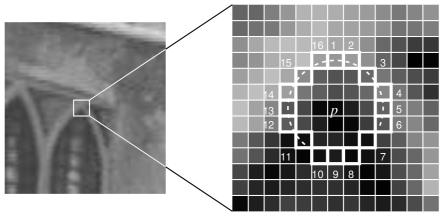
\includegraphics{fast_speedtest.jpg}

    \begin{Verbatim}[commandchars=\\\{\}]
{\color{incolor}In [{\color{incolor}23}]:} \PY{k}{def} \PY{n+nf}{circle}\PY{p}{(}\PY{n}{row}\PY{p}{,} \PY{n}{col}\PY{p}{)}\PY{p}{:}
             \PY{n}{point1} \PY{o}{=} \PY{p}{(}\PY{n}{row}\PY{o}{+}\PY{l+m+mi}{3}\PY{p}{,} \PY{n}{col}\PY{p}{)}
             
             \PY{n}{point2} \PY{o}{=} \PY{p}{(}\PY{n}{row}\PY{o}{+}\PY{l+m+mi}{3}\PY{p}{,} \PY{n}{col}\PY{o}{+}\PY{l+m+mi}{1}\PY{p}{)}
             
             \PY{n}{point3} \PY{o}{=} \PY{p}{(}\PY{n}{row}\PY{o}{+}\PY{l+m+mi}{2}\PY{p}{,} \PY{n}{col}\PY{o}{+}\PY{l+m+mi}{2}\PY{p}{)}
             
             \PY{n}{point4} \PY{o}{=} \PY{p}{(}\PY{n}{row}\PY{o}{+}\PY{l+m+mi}{1}\PY{p}{,} \PY{n}{col}\PY{o}{+}\PY{l+m+mi}{3}\PY{p}{)}
             
             \PY{n}{point5} \PY{o}{=} \PY{p}{(}\PY{n}{row}\PY{p}{,} \PY{n}{col}\PY{o}{+}\PY{l+m+mi}{3}\PY{p}{)}
             
             \PY{n}{point6} \PY{o}{=} \PY{p}{(}\PY{n}{row}\PY{o}{\PYZhy{}}\PY{l+m+mi}{1}\PY{p}{,} \PY{n}{col}\PY{o}{+}\PY{l+m+mi}{3}\PY{p}{)}
             
             \PY{n}{point7} \PY{o}{=} \PY{p}{(}\PY{n}{row}\PY{o}{\PYZhy{}}\PY{l+m+mi}{2}\PY{p}{,} \PY{n}{col}\PY{o}{+}\PY{l+m+mi}{2}\PY{p}{)}
             
             \PY{n}{point8} \PY{o}{=} \PY{p}{(}\PY{n}{row}\PY{o}{\PYZhy{}}\PY{l+m+mi}{3}\PY{p}{,} \PY{n}{col}\PY{o}{+}\PY{l+m+mi}{1}\PY{p}{)}
             
             \PY{n}{point9} \PY{o}{=} \PY{p}{(}\PY{n}{row}\PY{o}{\PYZhy{}}\PY{l+m+mi}{3}\PY{p}{,} \PY{n}{col}\PY{p}{)}
             
             \PY{n}{point10} \PY{o}{=} \PY{p}{(}\PY{n}{row}\PY{o}{\PYZhy{}}\PY{l+m+mi}{3}\PY{p}{,} \PY{n}{col}\PY{o}{\PYZhy{}}\PY{l+m+mi}{1}\PY{p}{)}
             
             \PY{n}{point11} \PY{o}{=} \PY{p}{(}\PY{n}{row}\PY{o}{\PYZhy{}}\PY{l+m+mi}{2}\PY{p}{,} \PY{n}{col}\PY{o}{\PYZhy{}}\PY{l+m+mi}{2}\PY{p}{)}
             
             \PY{n}{point12} \PY{o}{=} \PY{p}{(}\PY{n}{row}\PY{o}{\PYZhy{}}\PY{l+m+mi}{1}\PY{p}{,} \PY{n}{col}\PY{o}{\PYZhy{}}\PY{l+m+mi}{3}\PY{p}{)}
             
             \PY{n}{point13} \PY{o}{=} \PY{p}{(}\PY{n}{row}\PY{p}{,} \PY{n}{col}\PY{o}{\PYZhy{}}\PY{l+m+mi}{3}\PY{p}{)}
             
             \PY{n}{point14} \PY{o}{=} \PY{p}{(}\PY{n}{row}\PY{o}{+}\PY{l+m+mi}{1}\PY{p}{,} \PY{n}{col}\PY{o}{\PYZhy{}}\PY{l+m+mi}{3}\PY{p}{)}
             
             \PY{n}{point15} \PY{o}{=} \PY{p}{(}\PY{n}{row}\PY{o}{+}\PY{l+m+mi}{2}\PY{p}{,} \PY{n}{col}\PY{o}{\PYZhy{}}\PY{l+m+mi}{2}\PY{p}{)}
             
             \PY{n}{point16} \PY{o}{=} \PY{p}{(}\PY{n}{row}\PY{o}{+}\PY{l+m+mi}{3}\PY{p}{,} \PY{n}{col}\PY{p}{)}
             
             \PY{k}{return} \PY{p}{[}\PY{n}{point1}\PY{p}{,} \PY{n}{point2}\PY{p}{,} \PY{n}{point3}\PY{p}{,} \PY{n}{point4}\PY{p}{,} \PY{n}{point5}\PY{p}{,} \PY{n}{point6}\PY{p}{,} \PY{n}{point7}\PY{p}{,} \PY{n}{point8}\PY{p}{,} \PY{n}{point9}\PY{p}{,} \PY{n}{point10}\PY{p}{,} \PY{n}{point11}\PY{p}{,} \PY{n}{point12}\PY{p}{,} \PY{n}{point13}\PY{p}{,} \PY{n}{point14}\PY{p}{,} \PY{n}{point15}\PY{p}{]}
\end{Verbatim}


    \begin{Verbatim}[commandchars=\\\{\}]
{\color{incolor}In [{\color{incolor}24}]:} \PY{k}{def} \PY{n+nf}{is\PYZus{}corner}\PY{p}{(}\PY{n}{image}\PY{p}{,} \PY{n}{row}\PY{p}{,} \PY{n}{col}\PY{p}{,} \PY{n}{ROI}\PY{p}{,} \PY{n}{threshold}\PY{p}{,} \PY{n}{n\PYZus{}star}\PY{p}{)}\PY{p}{:}
             \PY{n}{intensity} \PY{o}{=} \PY{n+nb}{int}\PY{p}{(}\PY{n}{image}\PY{p}{[}\PY{n}{row}\PY{p}{]}\PY{p}{[}\PY{n}{col}\PY{p}{]}\PY{p}{)}
             \PY{n}{circ} \PY{o}{=} \PY{p}{[}\PY{p}{]}
             \PY{k}{for} \PY{n}{el} \PY{o+ow}{in} \PY{n}{ROI}\PY{p}{:}
                 \PY{k}{if} \PY{n}{image}\PY{p}{[}\PY{n}{el}\PY{p}{[}\PY{l+m+mi}{0}\PY{p}{]}\PY{p}{]}\PY{p}{[}\PY{n}{el}\PY{p}{[}\PY{l+m+mi}{1}\PY{p}{]}\PY{p}{]} \PY{o}{\PYZgt{}} \PY{n}{intensity}\PY{o}{+}\PY{n}{threshold}\PY{p}{:}
                     \PY{n}{circ}\PY{o}{.}\PY{n}{append}\PY{p}{(}\PY{l+m+mi}{1}\PY{p}{)}
                 \PY{k}{elif} \PY{n}{image}\PY{p}{[}\PY{n}{el}\PY{p}{[}\PY{l+m+mi}{0}\PY{p}{]}\PY{p}{]}\PY{p}{[}\PY{n}{el}\PY{p}{[}\PY{l+m+mi}{1}\PY{p}{]}\PY{p}{]} \PY{o}{\PYZlt{}} \PY{n}{intensity}\PY{o}{\PYZhy{}}\PY{n}{threshold}\PY{p}{:}
                     \PY{n}{circ}\PY{o}{.}\PY{n}{append}\PY{p}{(}\PY{l+m+mi}{2}\PY{p}{)}
                 \PY{k}{else}\PY{p}{:}
                     \PY{n}{circ}\PY{o}{.}\PY{n}{append}\PY{p}{(}\PY{l+m+mi}{0}\PY{p}{)}
             \PY{k}{for} \PY{n}{el} \PY{o+ow}{in} \PY{n}{ROI}\PY{p}{:}
                 \PY{k}{if} \PY{n}{image}\PY{p}{[}\PY{n}{el}\PY{p}{[}\PY{l+m+mi}{0}\PY{p}{]}\PY{p}{]}\PY{p}{[}\PY{n}{el}\PY{p}{[}\PY{l+m+mi}{1}\PY{p}{]}\PY{p}{]} \PY{o}{\PYZgt{}} \PY{n}{intensity}\PY{o}{+}\PY{n}{threshold}\PY{p}{:}
                     \PY{n}{circ}\PY{o}{.}\PY{n}{append}\PY{p}{(}\PY{l+m+mi}{1}\PY{p}{)}
                 \PY{k}{elif} \PY{n}{image}\PY{p}{[}\PY{n}{el}\PY{p}{[}\PY{l+m+mi}{0}\PY{p}{]}\PY{p}{]}\PY{p}{[}\PY{n}{el}\PY{p}{[}\PY{l+m+mi}{1}\PY{p}{]}\PY{p}{]} \PY{o}{\PYZlt{}} \PY{n}{intensity}\PY{o}{\PYZhy{}}\PY{n}{threshold}\PY{p}{:}
                     \PY{n}{circ}\PY{o}{.}\PY{n}{append}\PY{p}{(}\PY{l+m+mi}{2}\PY{p}{)}
                 \PY{k}{else}\PY{p}{:}
                     \PY{n}{circ}\PY{o}{.}\PY{n}{append}\PY{p}{(}\PY{l+m+mi}{0}\PY{p}{)}
             \PY{n}{i} \PY{o}{=}\PY{l+m+mi}{0}
             \PY{n}{el} \PY{o}{=} \PY{n}{circ}\PY{p}{[}\PY{n}{i}\PY{p}{]}
             \PY{n}{count} \PY{o}{=} \PY{l+m+mi}{1}
             \PY{n}{largest\PYZus{}ct} \PY{o}{=} \PY{n}{count}
             \PY{k}{for} \PY{n}{i} \PY{o+ow}{in} \PY{n+nb}{range}\PY{p}{(}\PY{l+m+mi}{1}\PY{p}{,} \PY{n+nb}{len}\PY{p}{(}\PY{n}{circ}\PY{p}{)}\PY{p}{)}\PY{p}{:}
                 \PY{k}{if} \PY{n}{circ}\PY{p}{[}\PY{n}{i}\PY{p}{]} \PY{o}{==} \PY{n}{el} \PY{o+ow}{and} \PY{n}{circ}\PY{p}{[}\PY{n}{i}\PY{p}{]} \PY{o}{!=} \PY{l+m+mi}{0}\PY{p}{:}
                     \PY{n}{count} \PY{o}{+}\PY{o}{=} \PY{l+m+mi}{1}
                 \PY{k}{else}\PY{p}{:}
                     \PY{k}{if} \PY{n}{circ}\PY{p}{[}\PY{n}{i}\PY{p}{]} \PY{o}{==} \PY{l+m+mi}{0}\PY{p}{:}
                         \PY{n}{el} \PY{o}{=} \PY{l+m+mi}{0}
                     \PY{k}{if} \PY{n}{circ}\PY{p}{[}\PY{n}{i}\PY{p}{]} \PY{o}{!=} \PY{l+m+mi}{0}\PY{p}{:}
                         \PY{k}{if} \PY{n}{largest\PYZus{}ct} \PY{o}{\PYZlt{}} \PY{n}{count}\PY{p}{:}
                             \PY{n}{largest\PYZus{}ct} \PY{o}{=} \PY{n}{count}
                         \PY{n}{count} \PY{o}{=} \PY{l+m+mi}{1}
                         \PY{n}{el} \PY{o}{=} \PY{n}{circ}\PY{p}{[}\PY{n}{i}\PY{p}{]}
         
             \PY{k}{return} \PY{n}{largest\PYZus{}ct} \PY{o}{\PYZgt{}}\PY{o}{=} \PY{n}{n\PYZus{}star}
\end{Verbatim}


    \begin{Verbatim}[commandchars=\\\{\}]
{\color{incolor}In [{\color{incolor}25}]:} \PY{k}{def} \PY{n+nf}{detect}\PY{p}{(}\PY{n}{image}\PY{p}{,} \PY{n}{threshold}\PY{o}{=}\PY{l+m+mi}{50}\PY{p}{)}\PY{p}{:}
             \PY{c+c1}{\PYZsh{} Initialization}
             \PY{n}{corners} \PY{o}{=} \PY{p}{[}\PY{p}{]}
             \PY{n}{rows}\PY{p}{,}\PY{n}{cols} \PY{o}{=} \PY{n}{image}\PY{o}{.}\PY{n}{shape}
             \PY{n}{startSearchRow} \PY{o}{=} \PY{l+m+mi}{3}
             \PY{n}{endSearchRow} \PY{o}{=} \PY{n}{rows}\PY{o}{\PYZhy{}}\PY{l+m+mi}{3}
             \PY{n}{startSearchCol} \PY{o}{=} \PY{l+m+mi}{3}
             \PY{n}{endSearchCol} \PY{o}{=} \PY{n}{cols}\PY{o}{\PYZhy{}}\PY{l+m+mi}{3}
             \PY{n}{n\PYZus{}star} \PY{o}{=} \PY{l+m+mi}{9}
         
             \PY{c+c1}{\PYZsh{} Begin searching through search area}
             \PY{k}{for} \PY{n}{row} \PY{o+ow}{in} \PY{n+nb}{range}\PY{p}{(}\PY{n}{startSearchRow}\PY{p}{,} \PY{n}{endSearchRow}\PY{p}{)}\PY{p}{:}
                 \PY{k}{for} \PY{n}{col} \PY{o+ow}{in} \PY{n+nb}{range}\PY{p}{(}\PY{n}{startSearchCol}\PY{p}{,} \PY{n}{endSearchCol}\PY{p}{)}\PY{p}{:}
                     \PY{n}{ROI} \PY{o}{=} \PY{n}{circle}\PY{p}{(}\PY{n}{row}\PY{p}{,} \PY{n}{col}\PY{p}{)} 
                     \PY{k}{if} \PY{n}{is\PYZus{}corner}\PY{p}{(}\PY{n}{image}\PY{p}{,} \PY{n}{row}\PY{p}{,} \PY{n}{col}\PY{p}{,} \PY{n}{ROI}\PY{p}{,} \PY{n}{threshold}\PY{p}{,} \PY{n}{n\PYZus{}star}\PY{p}{)}\PY{p}{:}
                         \PY{n}{corners}\PY{o}{.}\PY{n}{append}\PY{p}{(}\PY{p}{(}\PY{n}{col}\PY{p}{,} \PY{n}{row}\PY{p}{)}\PY{p}{)}
             \PY{k}{return} \PY{n}{corners}\PY{p}{;}
\end{Verbatim}


    \begin{Verbatim}[commandchars=\\\{\}]
{\color{incolor}In [{\color{incolor}26}]:} \PY{n}{tower} \PY{o}{=} \PY{n}{imread}\PY{p}{(}\PY{l+s+s1}{\PYZsq{}}\PY{l+s+s1}{./data/tower.png}\PY{l+s+s1}{\PYZsq{}}\PY{p}{)}
\end{Verbatim}


    \begin{Verbatim}[commandchars=\\\{\}]
{\color{incolor}In [{\color{incolor}27}]:} \PY{n}{thresholds} \PY{o}{=} \PY{p}{[}\PY{l+m+mi}{10}\PY{p}{,} \PY{l+m+mi}{20}\PY{p}{,} \PY{l+m+mi}{30}\PY{p}{,} \PY{l+m+mi}{50}\PY{p}{]}
         
         \PY{n}{plt}\PY{o}{.}\PY{n}{close}\PY{p}{(}\PY{l+s+s1}{\PYZsq{}}\PY{l+s+s1}{all}\PY{l+s+s1}{\PYZsq{}}\PY{p}{)}
         \PY{n}{f}\PY{p}{,} \PY{n}{axarr} \PY{o}{=} \PY{n}{plt}\PY{o}{.}\PY{n}{subplots}\PY{p}{(}\PY{l+m+mi}{1}\PY{p}{,} \PY{l+m+mi}{4}\PY{p}{,} \PY{n}{dpi}\PY{o}{=}\PY{l+m+mi}{200}\PY{p}{)}
         \PY{k}{for} \PY{n}{thresh} \PY{o+ow}{in} \PY{n}{thresholds}\PY{p}{:}
             \PY{n}{c} \PY{o}{=} \PY{n}{detect}\PY{p}{(}\PY{n}{tower}\PY{p}{,} \PY{n}{thresh}\PY{p}{)}
             \PY{n}{idx} \PY{o}{=} \PY{n}{thresholds}\PY{o}{.}\PY{n}{index}\PY{p}{(}\PY{n}{thresh}\PY{p}{)}
             \PY{n}{x\PYZus{}list} \PY{o}{=} \PY{p}{[}\PY{n}{x} \PY{k}{for} \PY{n}{x}\PY{p}{,} \PY{n}{y} \PY{o+ow}{in} \PY{n}{c}\PY{p}{]}
             \PY{n}{y\PYZus{}list} \PY{o}{=} \PY{p}{[}\PY{n}{y} \PY{k}{for} \PY{n}{x}\PY{p}{,} \PY{n}{y} \PY{o+ow}{in} \PY{n}{c}\PY{p}{]}
             \PY{n}{axarr}\PY{p}{[}\PY{n}{idx}\PY{o}{\PYZpc{}}\PY{k}{4}].axis(\PYZsq{}off\PYZsq{})
             \PY{n}{axarr}\PY{p}{[}\PY{n}{idx}\PY{o}{\PYZpc{}}\PY{k}{4}].scatter(x\PYZus{}list,y\PYZus{}list, s=0.5, color=\PYZsq{}green\PYZsq{})
             \PY{n}{axarr}\PY{p}{[}\PY{n}{idx}\PY{o}{\PYZpc{}}\PY{k}{4}].set\PYZus{}title(f\PYZsq{}\PYZdl{}T\PYZdl{} = \PYZob{}thresh\PYZcb{}\PYZsq{})
             \PY{n}{axarr}\PY{p}{[}\PY{n}{idx}\PY{o}{\PYZpc{}}\PY{k}{4}].imshow(tower, cmap=\PYZsq{}gray\PYZsq{})
\end{Verbatim}


    \begin{center}
    \adjustimage{max size={0.9\linewidth}{0.9\paperheight}}{output_38_0.png}
    \end{center}
    { \hspace*{\fill} \\}
    
    We notice that our FAST detector performs similar to the ones on slides,
and also similar to the standard library implementation (given below).
This is suprising because the standard library version uses a fast
approximation where it only checks a select ``points'' that were
pre-determined to be useful instead of checking if the entire array
passes the \(n^*\) test like we do. (This version also is noticeably
faster because of less looping and branching required along with lesser
memory overhead as the amount of points required in this method is
nearly half.

    \hypertarget{bonus-comparision-with-standard-library-results}{%
\section{Bonus comparision with standard library
results}\label{bonus-comparision-with-standard-library-results}}

    \begin{Verbatim}[commandchars=\\\{\}]
{\color{incolor}In [{\color{incolor}28}]:} \PY{k+kn}{from} \PY{n+nn}{skimage}\PY{n+nn}{.}\PY{n+nn}{feature} \PY{k}{import} \PY{n}{corner\PYZus{}harris}\PY{p}{,} \PY{n}{corner\PYZus{}fast}\PY{p}{,} \PY{n}{corner\PYZus{}subpix}\PY{p}{,} \PY{n}{corner\PYZus{}peaks}\PY{p}{,} \PY{n}{corner\PYZus{}shi\PYZus{}tomasi}
         \PY{n}{coords} \PY{o}{=} \PY{n}{corner\PYZus{}peaks}\PY{p}{(}\PY{n}{corner\PYZus{}harris}\PY{p}{(}\PY{n}{checker}\PY{p}{)}\PY{p}{,} \PY{n}{min\PYZus{}distance}\PY{o}{=}\PY{l+m+mi}{1}\PY{p}{)}
         \PY{n}{coords\PYZus{}subpix} \PY{o}{=} \PY{n}{corner\PYZus{}subpix}\PY{p}{(}\PY{n}{checker}\PY{p}{,} \PY{n}{coords}\PY{p}{,} \PY{n}{window\PYZus{}size}\PY{o}{=}\PY{l+m+mi}{1}\PY{p}{)}
         \PY{n}{fig}\PY{p}{,} \PY{n}{ax} \PY{o}{=} \PY{n}{plt}\PY{o}{.}\PY{n}{subplots}\PY{p}{(}\PY{p}{)}
         \PY{n}{ax}\PY{o}{.}\PY{n}{imshow}\PY{p}{(}\PY{n}{checker}\PY{p}{,} \PY{n}{interpolation}\PY{o}{=}\PY{l+s+s1}{\PYZsq{}}\PY{l+s+s1}{nearest}\PY{l+s+s1}{\PYZsq{}}\PY{p}{,} \PY{n}{cmap}\PY{o}{=}\PY{l+s+s1}{\PYZsq{}}\PY{l+s+s1}{copper}\PY{l+s+s1}{\PYZsq{}}\PY{p}{)}
         \PY{n}{ax}\PY{o}{.}\PY{n}{axis}\PY{p}{(}\PY{l+s+s1}{\PYZsq{}}\PY{l+s+s1}{off}\PY{l+s+s1}{\PYZsq{}}\PY{p}{)}
         \PY{n}{ax}\PY{o}{.}\PY{n}{plot}\PY{p}{(}\PY{n}{coords}\PY{p}{[}\PY{p}{:}\PY{p}{,} \PY{l+m+mi}{1}\PY{p}{]}\PY{p}{,} \PY{n}{coords}\PY{p}{[}\PY{p}{:}\PY{p}{,} \PY{l+m+mi}{0}\PY{p}{]}\PY{p}{,} \PY{l+s+s1}{\PYZsq{}}\PY{l+s+s1}{.b}\PY{l+s+s1}{\PYZsq{}}\PY{p}{,} \PY{n}{c}\PY{o}{=}\PY{l+s+s1}{\PYZsq{}}\PY{l+s+s1}{aqua}\PY{l+s+s1}{\PYZsq{}}\PY{p}{,} \PY{n}{markersize}\PY{o}{=}\PY{l+m+mi}{3}\PY{p}{)}
         \PY{n}{plt}\PY{o}{.}\PY{n}{show}\PY{p}{(}\PY{p}{)}
\end{Verbatim}


    \begin{center}
    \adjustimage{max size={0.9\linewidth}{0.9\paperheight}}{output_41_0.png}
    \end{center}
    { \hspace*{\fill} \\}
    
    We notice that they get results that we got earlier (with R), but since
they haven't applied our variation of non-maximal suppression they loose
some of the lower corners.

    \begin{Verbatim}[commandchars=\\\{\}]
{\color{incolor}In [{\color{incolor}29}]:} \PY{n}{coords} \PY{o}{=} \PY{n}{corner\PYZus{}peaks}\PY{p}{(}\PY{n}{corner\PYZus{}shi\PYZus{}tomasi}\PY{p}{(}\PY{n}{checker}\PY{p}{)}\PY{p}{,} \PY{n}{min\PYZus{}distance}\PY{o}{=}\PY{l+m+mi}{1}\PY{p}{)}
         \PY{n}{coords\PYZus{}subpix} \PY{o}{=} \PY{n}{corner\PYZus{}subpix}\PY{p}{(}\PY{n}{checker}\PY{p}{,} \PY{n}{coords}\PY{p}{,} \PY{n}{window\PYZus{}size}\PY{o}{=}\PY{l+m+mi}{1}\PY{p}{)}
         \PY{n}{fig}\PY{p}{,} \PY{n}{ax} \PY{o}{=} \PY{n}{plt}\PY{o}{.}\PY{n}{subplots}\PY{p}{(}\PY{p}{)}
         \PY{n}{ax}\PY{o}{.}\PY{n}{imshow}\PY{p}{(}\PY{n}{checker}\PY{p}{,} \PY{n}{interpolation}\PY{o}{=}\PY{l+s+s1}{\PYZsq{}}\PY{l+s+s1}{nearest}\PY{l+s+s1}{\PYZsq{}}\PY{p}{,} \PY{n}{cmap}\PY{o}{=}\PY{l+s+s1}{\PYZsq{}}\PY{l+s+s1}{copper}\PY{l+s+s1}{\PYZsq{}}\PY{p}{)}
         \PY{n}{ax}\PY{o}{.}\PY{n}{axis}\PY{p}{(}\PY{l+s+s1}{\PYZsq{}}\PY{l+s+s1}{off}\PY{l+s+s1}{\PYZsq{}}\PY{p}{)}
         \PY{n}{ax}\PY{o}{.}\PY{n}{plot}\PY{p}{(}\PY{n}{coords}\PY{p}{[}\PY{p}{:}\PY{p}{,} \PY{l+m+mi}{1}\PY{p}{]}\PY{p}{,} \PY{n}{coords}\PY{p}{[}\PY{p}{:}\PY{p}{,} \PY{l+m+mi}{0}\PY{p}{]}\PY{p}{,} \PY{l+s+s1}{\PYZsq{}}\PY{l+s+s1}{.b}\PY{l+s+s1}{\PYZsq{}}\PY{p}{,} \PY{n}{c}\PY{o}{=}\PY{l+s+s1}{\PYZsq{}}\PY{l+s+s1}{aqua}\PY{l+s+s1}{\PYZsq{}}\PY{p}{,} \PY{n}{markersize}\PY{o}{=}\PY{l+m+mi}{3}\PY{p}{)}
         \PY{n}{plt}\PY{o}{.}\PY{n}{show}\PY{p}{(}\PY{p}{)}
\end{Verbatim}


    \begin{center}
    \adjustimage{max size={0.9\linewidth}{0.9\paperheight}}{output_43_0.png}
    \end{center}
    { \hspace*{\fill} \\}
    
    The Shi-Tomasi corner detector gives us results comparable to our
implementation of Harris.

    \begin{Verbatim}[commandchars=\\\{\}]
{\color{incolor}In [{\color{incolor}30}]:} \PY{n}{coords} \PY{o}{=} \PY{n}{corner\PYZus{}peaks}\PY{p}{(}\PY{n}{corner\PYZus{}fast}\PY{p}{(}\PY{n}{tower}\PY{p}{,} \PY{l+m+mi}{10}\PY{p}{)}\PY{p}{,} \PY{n}{min\PYZus{}distance}\PY{o}{=}\PY{l+m+mi}{1}\PY{p}{)}
         \PY{n}{coords\PYZus{}subpix} \PY{o}{=} \PY{n}{corner\PYZus{}subpix}\PY{p}{(}\PY{n}{tower}\PY{p}{,} \PY{n}{coords}\PY{p}{,} \PY{n}{window\PYZus{}size}\PY{o}{=}\PY{l+m+mi}{3}\PY{p}{)}
         \PY{n}{fig}\PY{p}{,} \PY{n}{ax} \PY{o}{=} \PY{n}{plt}\PY{o}{.}\PY{n}{subplots}\PY{p}{(}\PY{p}{)}
         \PY{n}{ax}\PY{o}{.}\PY{n}{imshow}\PY{p}{(}\PY{n}{tower}\PY{p}{,} \PY{n}{interpolation}\PY{o}{=}\PY{l+s+s1}{\PYZsq{}}\PY{l+s+s1}{nearest}\PY{l+s+s1}{\PYZsq{}}\PY{p}{,} \PY{n}{cmap}\PY{o}{=}\PY{n}{plt}\PY{o}{.}\PY{n}{cm}\PY{o}{.}\PY{n}{gray}\PY{p}{)}
         \PY{n}{ax}\PY{o}{.}\PY{n}{plot}\PY{p}{(}\PY{n}{coords}\PY{p}{[}\PY{p}{:}\PY{p}{,} \PY{l+m+mi}{1}\PY{p}{]}\PY{p}{,} \PY{n}{coords}\PY{p}{[}\PY{p}{:}\PY{p}{,} \PY{l+m+mi}{0}\PY{p}{]}\PY{p}{,} \PY{l+s+s1}{\PYZsq{}}\PY{l+s+s1}{.}\PY{l+s+s1}{\PYZsq{}}\PY{p}{)}
         \PY{n}{ax}\PY{o}{.}\PY{n}{axis}\PY{p}{(}\PY{l+s+s1}{\PYZsq{}}\PY{l+s+s1}{off}\PY{l+s+s1}{\PYZsq{}}\PY{p}{)}
         \PY{n}{plt}\PY{o}{.}\PY{n}{show}\PY{p}{(}\PY{p}{)}
\end{Verbatim}


    \begin{center}
    \adjustimage{max size={0.9\linewidth}{0.9\paperheight}}{output_45_0.png}
    \end{center}
    { \hspace*{\fill} \\}
    
    Fairly similar results at similar threshold as our implementation, but
at a fraction of the computational overhead. Argument could be made
about it tripping up on some more complex image.


    % Add a bibliography block to the postdoc
    
    
    
    \end{document}
